\documentclass[12pt]{exam}
\usepackage{amsthm}
\usepackage{libertine}
\usepackage[utf8]{inputenc}
\usepackage[margin=1in]{geometry}
\usepackage{amsmath,amssymb}
\usepackage{multicol}
\usepackage[shortlabels]{enumitem}
\usepackage{siunitx}
\usepackage{cancel}
\usepackage{caption}
\usepackage{graphicx}
\usepackage{pgfplots}
\usepackage{listings}
\usepackage{tikz}


\pgfplotsset{width=10cm,compat=1.9}
\usepgfplotslibrary{external}
\tikzexternalize

\newcommand{\class}{Laboratorio Ondas y Fluidos} % This is the name of the course 
\newcommand{\examnum}{Laboratorio $0$} % This is the name of the assignment
\newcommand{\examdate}{01/02/2023} % This is the due date
\newcommand{\timelimit}{}
\newenvironment{Figura}
  {\par\medskip\noindent\minipage{\linewidth}}
  {\endminipage\par\medskip}




\begin{document}
\pagestyle{plain}
\thispagestyle{empty}

\noindent
\begin{tabular*}{\textwidth}{l @{\extracolsep{\fill}} r @{\extracolsep{6pt}} l}
  \textbf{\class} & \textbf{Name:} &  \textit{Mauricio Devia}\\
  \textbf{\examnum} &&\textit{Sergio Montoya Ramírez}\\
\textbf{\examdate} &&\\
\end{tabular*}\\
\rule[2ex]{\textwidth}{2pt}
% ---


\begin{multicols}{2}
\section{Objetivos}
\begin{itemize}
\item Dadas variables con medidas e incertidumbres, propagar errores.
\item Por medio de las herramientas de \textit{Logger Pro}, realizar un ajuste y regresión lineal.
\item Hacer gráficas de datos importados.
\end{itemize}
\section{Introducción}
Los instrumentos de medida no son perfectos de manera que al medir una longitud con una regla y ver que la regla esta marcando 8.7 cm habrá cierta incertidumbre de medida, ya que bien podría ser que su verdadera medida es un poco mayor o menor del valor que estamos viendo. Por lo tanto, para tener esto en consideración al realizar una practica de laboratorio lo que se hace es expresar estos valores de la forma $$(m \pm n)$$ en donde m es el valor hallado y n la incertidumbre.
\section{Teoría}
\subsection*{Propagación de Errores}
Si debemos determinar el valor de una variable que involucra la medida de distintas variables, los instrumentos que se usaron pueden tener incluso incertidumbres diferentes. Por lo tanto para encontrar la incertidumbre real se debe propagar el error. Para encontrar el valor de esta propagación se hace lo siguiente.

  Dadas n diferentes mediciones representadas por $x_i$ con sus respectivas incertidumbres $\sigma_{xi}$ , de manera que las variables $x_i$ se relacionan con una función matemática $f = f(x_1,x_2,x_3,...,x_n);$ entonces la incertidumbre para f va a ser:

  $$\sigma_f = \sqrt{\left(\frac{\partial f}{\partial x_1}\sigma_{x1}\right)^2+...+\left(\frac{\partial f}{\partial x_n}\sigma_{x_n}\right)^2}$$

  \subsection{Ajustes}
  En un experimento en el que se han realizado n medidas para dos variables x y y de las que si se realiza una gráfica se ve que tiene una tendencia definida, es posible encontrar una función que se ajuste de la mejor manera a los puntos sobre la gráfica. Ajustar una recta se conoce como \textbf{Regresión Lineal}.
  \section{Ejercicios}
  \subsection{Ajuste}
  \begin{Figura}
    \centering
    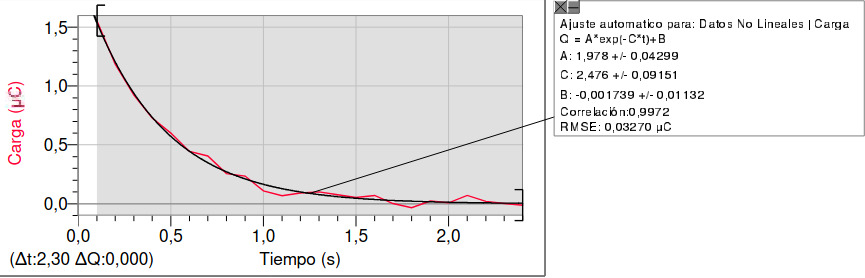
\includegraphics[width=0.9\textwidth]{Imagen_1.jpeg}
    \captionof{figure}{Ajuste no lineal para la regreción de los datos dados en el experimento}
    \label{fig}
\end{Figura}
  \begin{tabular}{|ccc|}
    \hline
    A & = & $(1.98 \pm 0.04)$\\
    D & = & $(2.48 \pm 0.09)$\\
    B & = & $(-0.002 \pm 0.01)$\\
    \hline
\end{tabular}
  \subsection{Propagación de Error}
  \begin{tabular}{|ccc|}
    Resistencia Experimental & = & $(2.016 \pm 7316)\times 10^{5}$\\
    Resistencia Real & = & $(200 \pm 10)\times 10^3$\\
  \end{tabular}
  Se acomodaron las unidades puesto que estas se enncontraban en unidades distintas y al hacer esto nos damos cuenta que ambas resistencias comparten un espacio en su intervalo y  por tanto es exacto. Sin embargo, dada la incertidumbre tan alta no podriamos llamarlo preciso.
  \subsection{Linealización}
  \begin{Figura}
    \centering
    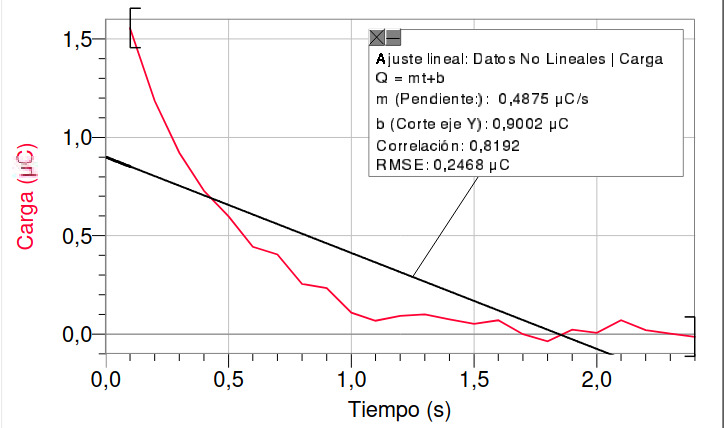
\includegraphics[width=0.9\textwidth]{Imagen_2.jpeg}
    \captionof{figure}{Ajuste lineal para la regreción de los datos dados en el experimento}
    \label{fig}
\end{Figura}
  \subsection{Fourier}
\begin{Figura}
    \centering
    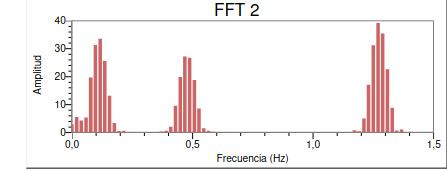
\includegraphics[width=0.9\textwidth]{Imagen_3.jpeg}
    \captionof{figure}{Factorización en serie de Fourier de la grafica dada en el ejercicio}
    \label{fig}
\end{Figura}
  \subsubsection{Primer Pico:}
  \begin{eqnarray*}
    A & = & 0.35 m\\
    f & = & 0.12 Hz\\
    T & = & 8.33 s\\
    \omega & = & 0.75 \frac{rad}{s}\\
    f(t) & = & 0.35\sin(0.75t)
  \end{eqnarray*}
  \subsubsection{Segundo Pico}
   \begin{eqnarray*}
    A & = & 0.27 m\\
    f & = & 0.48 Hz\\
    T & = & 2.08 s\\
    \omega & = & 3.02 \frac{rad}{s}\\
    f(t) & = & 0.27\sin(3.02t)
  \end{eqnarray*}
  \subsubsection{Tercer Pico}
   \begin{eqnarray*}
    A & = & 0.40 m\\
    f & = & 1.28 Hz\\
    T & = & 0.78 s\\
    \omega & = & 8.10 \frac{rad}{s}\\
    f(t) & = & 0.40\sin(8.10t)
  \end{eqnarray*}
  \subsubsection{Función}
  $$f(t) = A_1\sin(\omega_1t) + A_2\sin(\omega_2t) + A_3\sin(\omega_3t)$$
  $$f(t) = 0.35\sin(0.75t) + 0.27\sin(3.02t) + 0.40\sin(8.10t)$$
\end{multicols}

\end{document}
